In the following, SLIM is used in different configurations as a surrogate for modelling the benefit present values of two insurance tariffs. The results are interpreted and the fidelity is compared with the MBT algorithms GUIDE, MOB and CTree.

\subsection{Data set K2204}
The data set K2204 contains data for a (fictitious) endowment insurance tariff and includes the features sex, age and duration and the two targets benefit present value (BPV) and premium present value (PPV). The targets were modelled using two different black box models.  
In the following, only the BPV is considered. The results for the PBV are very similar (interpreted the other way round) and can be found in the appendix. A special characteristic of this data set is a correlation between the Age and Duration features, as can be seen in Figure \ref{fig:ins_corr_age_duration}. When interpreting a MBT for this data set, it must therefore be taken into account that a split with regard to one of the features always has an influence on the value range of the other feature.

\begin{figure}[!htb]
    \centering    
    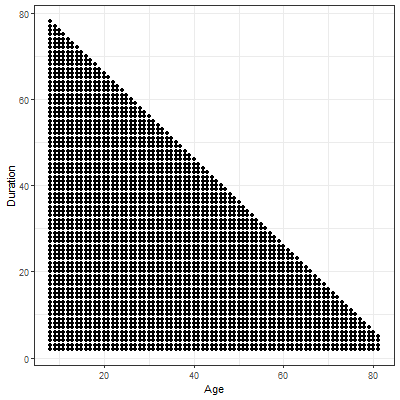
\includegraphics[width=7cm]{Figures/insurance_use_case/k2204_BPV/corr_age_duration.png}
    \caption{Features Age and Duration in the K2204 data set}
    \label{fig:ins_corr_age_duration}
\end{figure}

In a first step, SLIM was fitted as surrogate to the black box predictions of BPV (BPV\_pred) with linear regression models in the nodes. The maximum depth was set to 3 and an improvement in the objective of at least 0.1 of the previous improvement was set as prepruning parameter.
 The resulting tree is shown in Figure \ref{fig:ins_slim_lm_tree}.

 \begin{figure}[!htb]
     \centering     
     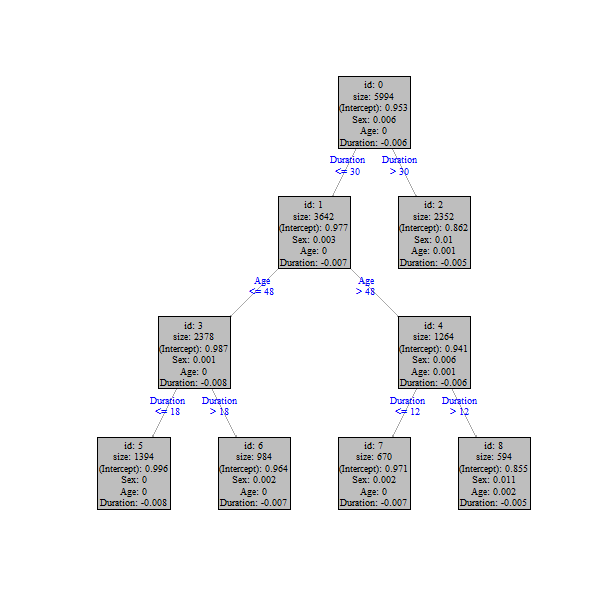
\includegraphics[width = 14cm]{Figures/insurance_use_case/k2204_BPV/slim_lm_tree.png}
     \caption{SLIM tree for K2204 with linear models}
     \label{fig:ins_slim_lm_tree}
 \end{figure}

Basic observations across all subregions are:
\begin{itemize}
    \item Gender male has a positive effect on BPV\_pred
    \item Age has a positive effect on BPV\_pred
    \item Duration has a negative effect on BPV\_pred
\end{itemize}

The strength of the effects, however, differs in the different subregions found by SLIM.
The five leafnodes can be roughly divided into two regions with similar effects:
\begin{itemize}
    \item Region 1 (Nodes 2,8): High Duration ($30$) or high Age ($>48$) and medium Duration (between $13$ and $30$)
    \item Region 2 (Nodes 5,6,7): Low - medium Duration with low Age or high Age with low Duration ($\leq 12$)
\end{itemize}

In Region 1 Sex male and Age have a higher positive effect on  BPV\_pred than in region 2. The negative effect of duration, on the other hand, is smaller in region 1. This indicates a non-linearity of duration.

If SLIM is fitted as a standalone model instead of a surrogate model in the same configuration, the differences in the split points are very small. This indicates that the black box model captures the underlying relationships very well. The corresponding tree is shown in the appendix in Figure \ref{}.

\subsection{Data set R108}